%% LyX 2.0.5.1 created this file.  For more info, see http://www.lyx.org/.
%% Do not edit unless you really know what you are doing.
\documentclass[english]{article}
\usepackage[T1]{fontenc}
\usepackage[latin9]{inputenc}
\usepackage{units}
\usepackage{amssymb}
\usepackage{graphicx}

\makeatletter

%%%%%%%%%%%%%%%%%%%%%%%%%%%%%% LyX specific LaTeX commands.
\newcommand{\noun}[1]{\textsc{#1}}

%%%%%%%%%%%%%%%%%%%%%%%%%%%%%% User specified LaTeX commands.
\usepackage{bbm}

\date{May $14^{th}$ 2013}

\@ifundefined{showcaptionsetup}{}{%
 \PassOptionsToPackage{caption=false}{subfig}}
\usepackage{subfig}
\makeatother

\usepackage{babel}
\begin{document}

\title{Architectural Morphology\\
Investigative modeling and spatial analysis}

\maketitle
\bigskip{}
\bigskip{}
\bigskip{}


\textit{\large \hfill{}Public Research Workshop\hfill{}\hfill{}}{\large \par}

\textit{\large \hfill{}Stockholm, KTH School of Architecture\hfill{}\hfill{}}{\large \par}

\bigskip{}
\bigskip{}
\bigskip{}
\bigskip{}

\begin{abstract}
The development of new theorical and technical means, particularly
in the field of computer science and its direct applications, leads
more and more to a renewal of the approach on design and architecture.
The increasing place of modeling and calculations in the architectural
process confirms that Architecture lays on the interface, in this
case ambiguous, between art and science.
\end{abstract}
\newpage{}

\textit{\large \hfill{}}\textbf{\Large Speakers}\textit{\large \hfill{}\hfill{}}{\large \par}

\bigskip{}
\bigskip{}


\textit{\large \hfill{}}\noun{John Peponis}\textit{\large \hfill{}\hfill{}}{\large \par}

\textit{\large \hfill{}}Professor, Associate Chair Advanced Studies
and Research\textit{\large \hfill{}\hfill{}}{\large \par}

\textit{\large \hfill{}}GeorgiaTech School of Architecture\textit{\large \hfill{}\hfill{}}{\large \par}

\bigskip{}


\textit{\large \hfill{}}\noun{Sophia Psarra}\textit{\large \hfill{}\hfill{}}{\large \par}

\textit{\large \hfill{}}Reader of Architecture and Spatial Design\textit{\large \hfill{}\hfill{}}{\large \par}

\textit{\large \hfill{}}The Bartlett School of Graduate Studies,
Editor, Journal of Space Syntax\textit{\large \hfill{}\hfill{}}{\large \par}

\bigskip{}


\textit{\large \hfill{}}\noun{Ermal Shpuza}\textit{\large \hfill{}\hfill{}}{\large \par}

\textit{\large \hfill{}}Associate Professor\textit{\large \hfill{}\hfill{}}{\large \par}

\textit{\large \hfill{}}Department of Architecture, Southern Polytechnic
State University\textit{\large \hfill{}\hfill{}}{\large \par}

\bigskip{}


\textit{\large \hfill{}}\noun{Meta Berghauser Pont}\textit{\large \hfill{}\hfill{}}{\large \par}

\textit{\large \hfill{}}Chair Urban Design \textendash{} Theory and
Methods\textit{\large \hfill{}\hfill{}}{\large \par}

\textit{\large \hfill{}}TU Delft Faculty of Architecture\textit{\large \hfill{}\hfill{}}{\large \par}

\bigskip{}


\textit{\large \hfill{}}\noun{Ulrika Karlsson}\textit{\large \hfill{}\hfill{}}{\large \par}

\textit{\large \hfill{}}Visiting Professor School of Architecture,
KTH; servo stockholm\textit{\large \hfill{}\hfill{}}{\large \par}

\bigskip{}


\textit{\large \hfill{}}\noun{Christian Deri}\textit{\large \hfill{}\hfill{}}{\large \par}

\textit{\large \hfill{}}Head of AEDAS Architects R\&D\textit{\large \hfill{}\hfill{}}{\large \par}

\textit{\large \hfill{}}Visiting Professor, Technical University
of Munich\textit{\large \hfill{}\hfill{}}{\large \par}

\bigskip{}


\textit{\large \hfill{}}\noun{�smund Izaki}\textit{\large \hfill{}\hfill{}}{\large \par}

\textit{\large \hfill{}}AEDAS Architects R\&D\textit{\large \hfill{}\hfill{}}{\large \par}

\bigskip{}


\textit{\large \hfill{}}\noun{Daniel Koch}\textit{\large \hfill{}\hfill{}}{\large \par}

\textit{\large \hfill{}}Researcher, Director of Research Studies\textit{\large \hfill{}\hfill{}}{\large \par}

\textit{\large \hfill{}}KTH School of Architecture\textit{\large \hfill{}\hfill{}}{\large \par}

\bigskip{}


\textit{\large \hfill{}}\noun{Pablo Miranda Carranza}\textit{\large \hfill{}\hfill{}}{\large \par}

\textit{\large \hfill{}}Researcher\textit{\large \hfill{}\hfill{}}{\large \par}

\textit{\large \hfill{}}KTH School of Architecture\textit{\large \hfill{}\hfill{}}{\large \par}

\newpage{}


\section*{Introduction\bigskip{}
\bigskip{}
}

\textit{This workshop was presented as follows :}

\bigskip{}


\bigskip{}


The Research Workshop Architectural Morphology: Investigative modeling
and spatial analysis is meant as a beginning or a point of departure,
in research and for coming events revolving around modeling and spatial
analysis in architecture. With speakers of considerable repute within
the field commonly referred to as Space Syntax, as well as in other
Architectural fields, it is meant to communicate cutting edge analytical,
configurative modeling as well as explore relations to other modeling
and analytical traditions in architectural research. Furthermore,
through the participation of AEDAS R\&D and the experience of many
of the speakers, the relation between modeling and analysis in research
and practice will be highlighted and discussed.

\newpage{}


\section*{\noun{John Peponis}, GeorgiaTech School of Architecture\protect \\
Concrete applications of Space Syntax}

We unfortunately missed the begining of this first presentation.

That presented direct application of spatial integration calculations
on Atlanta districts.

{[}explanation schema and formulas{]}

It is possible for example, by distinguishing pedestrian and car axial
maps, to show evidences of ``bad'' designed district in the sense
that they are not liveable for a pedestrian, what is no more possible
nowadays. Such designs present a strong lack of flexibility.

Such errors could have been avoided by the use of analytic methods
like spatial analysis, and we need today to switch from an exclusive
descriptive approach of architecture to a normative point of view
; we need more normative, evidence-based practice. For example, back
to the Atlanta districts, it can be showed through investigative modeling
that a greater building flexibility could have been permitted thanks
to a non equivalent distribution of block size ; that can be put in
parallel with the need for local activity diversification.

Of course spatial analysis will never be the direct answer to the
difficult question of what is an ideal city, but the motivation of
space syntax has always been a normative aim through a better understanding
of urban systems

\newpage{}


\section*{\noun{Sophia Psarra}, UCL\protect \\
The Venice variations : Interactions between generation and explanation}


\subsection*{1 Role of spatial analysis considerations in Design and Architectural
Knowledge}

Architecture and its narrative approach are direct consequences of
the geometric spatial configuration and an embodied experience, which
can be approximated through a topological description of space. That's
why geometry and topology play both key roles in architectural analysis
; they have in fact a strong relationship which form determine most
aspects of the architectural experience.

As a consequence, a useful tool of investigative modeling can be the
try of different geometric shapes associated with the same topology.
In that case, whereas the spatial integration stays the same (since
we define it in the classic way, with $N$ places and $d_{ij}$ the
topological distance from place $i$ to $j$, the mean accessibility
to other places : $I_{S}=\frac{2}{N\cdot(N-1)}\cdot\sum_{i<j}d_{ij}$
) because it depends only of the topological configuration, the visual
integration differs and is interesting to consider as a design criteria.
The visual integration can be defined as follows : the architectural
structure can be considered as a subset $A\subset P\subset\mathbb{R}^{2}$,
where $P$ is the part of the space we work in. Then the visual integration
of a point is the measure of the visually accessible subset taking
into account the architectural obstacles (walls). For $M\in P$, it
is defined as \[I_{v}(M)=\intop_{M'\in P \backslash S}{\mathbbm{1}_{\{M+t \vec{MM'}|t\in [0,1]\} \cap S = \emptyset} dS}\]

Such a criteria can also be generalised in 3 dimensions, by discrete
superposition of floor layers, or by an analog continuous definition.

Its use can then play role in the development of architectural knowledge.
In \cite{calvino1978invisible}, \noun{Calvino} explains that imagination
can be in fact considered as \textit{Ars combinatoria}, that means
finding one good configuration among all possibles. In other words,
creating is exploring the plurality of words. The knowledge can be
classified in 4 types : dialectic knowledge (empirical), encyclopedic
knowledge (to make predictions), analytic knowledge (calculations)
and creative knowledge (imagination) ; and design is in particular
the combination of the last two : it joins these two different types
of knowledge through functionnal aspect and the use of imagination.

To go further in the role of computation in design, we can consider
the work of Smithson in the 70s, and the concept of ``Mat-building''
developped particularly in \cite{smithson1974recognize}. The important
ideas are that architecture and urbanism are closely linked to the
notion of emergence, and that an only top-down approach is not sufficient,
a bottom-up approach is also needed, by considerations of evolutionnary
fields and local relations.

That importance of computers in design was later in the 90s confirmed
by the apparition of evolutionnal design, e. g. design through genetic
algorithm that use given rules of the genetic languages to compute
new designs. That is again a bottom-up approach for which the unpredictability
of the emerging properties is inherent to the system and its self-organisation.


\subsection*{2 Evolution and Urban form : case Venice}


\subsection*{3 Comparison to the project of hospital by Le Corbusier}


\subsection*{4 Consequences on design}

\newpage{}


\section*{\noun{Daniel Koch}, KTH\protect \\
Architectural Interfaces \& Resilience}


\subsection*{Introduction}

Architecture can be seen as the interface between the one and other
: it has a strong impact on the social relations. Whereas socio-cultural
identification can explain differences in housings, on the opposite
how is architecture communicating with these socio-cultural considerations?


\subsection*{Characterization of interfaces}


\subsection*{Consequences for the resilience of the built environment}

\newpage{}


\section*{\noun{Pablo Miranda Carranza}, KTH\protect \\
Tools used nowadays in advanced spatial analysis}


\subsection*{Generalities}


\subsection*{Analysis of bunker architecture through convex decomposition of space}

\newpage{}


\section*{\noun{Meta Berghauser Pont}, TU Delft\protect \\
Density, Architecture and the City}


\subsection*{Why study density?}

Through history, density of cities has always have a great importance.
As a concrete example, there is evidence of the link between a high
density of population and health problems in Ansterdam, Jordean at
the end of the 19th century. At the same time, regulations to constraint
the height of buildings according to the street width were taken all
over the world (see Paris of \noun{Haussman} for example). The promoters
of the Garden City took the aspect of a healthier city as a main argument.
In the late 50s, Jacobs proposed (\cite{Jac56}) in opposition to
these idealisms a return to a more natural and by consequence a more
dense city.

Today, density can still be an issue. Back to the example of Amsterdam,
the global density is too low, as a consequence of an explosion of
the urban footprint, and of different relative growths of land uses
(the proportion of dwellings went bigger).

We could try to give an answer to the question of arguments for or
against densification, but there are very much pertinent arguments
on both side, so the really important aspect that appears is the study
of density in itself, the fact that it has good or bad consequences
on some aspects of the urban system is in fact an other problem, depending
most of the time on the particular concrete situation we are in.


\subsection*{Measuring density}


\subsection*{Performance of density}

\newpage{}


\section*{\noun{Ermal Shpuza}, Southern Polytechnic State University\protect \\
Interaction between boundary shape and circulation structure in the
built environment}

Recent research work has been oriented towards the study of the mutual
effect of rules and constraints, in the sense of the relations between
the building shape and the social organization occupying it. These
two elements have totally different time longevity, so we can ask
if it could lead to contradictions between the functionnal aim of
an architecture and its effective use.

That lead to the study of two aspects and the links they have : the
boudary shape of the building and the contained circulation. Circulation
system is directly linked to a level of movement, and can be taken
as a local description of floorplates, whereas the boundaries are
more a global description. Such a study can also be done at the urban
scale, by searching the impacts of an imposed shape on internal circulations.

We will see here first the pure shape aspect, then the influence of
circulation on shape, and finally the inverse relation.


\subsection*{1 Unique shape approach}

It can be useful to first describe the boundary shape in itself, since
we will interest us later on clustering of shapes.

Given a boundary shape, it is possible to extract a polygonal approximation
(which can be exact in the case of a polygonal shape, what is the
most used case for the following studies), and then classify it through
the classification of the polygon.

It has been shown ({[}Missing reference{]}) that a polygonal shape
can be quite uniquely put in correspondance with 6 sets of reals numbers,
that are, if we note, with $S$ summits of the polygons, $A_{i}(s)$
the set of depth $i$ adjacent summits to summit $s$, $S_{i}^{j}=\{d(k,a)^{j}|k\in S,a\in A_{i}(k)\}$,
the particular sets $S_{1}^{1}$, $S_{2}^{1}$, $S_{3}^{1}$, $S_{1}^{2}$,
$S_{2}^{2}$ and $S_{3}^{2}$.

Such a classification of polygonal shapes is the starting point of
the following work, since we will work on unscaled polygonal shapes,
i.e. with $\mathcal{P}$ set of polygonal shape and the equivalence
relation on it : $\mathcal{R}:P_{1}\mathcal{R}P_{2}\iff(\exists\alpha\in\mathbb{R}^{*},S_{i}^{j}(P_{1})=\alpha S_{i}^{j}(P_{2}),i=1,2,3,j=1,2)$
, on the quotient set $\nicefrac{\mathcal{P}}{\mathcal{R}}$. On the
following, when we consider polygonal shapes, it will always be on
that set.


\subsection*{2 From circulation to shape : the inside-out approach}

This approach is a modular approach, in the sense that it goes from
inside to outside. The internal space influences the boundary shape.
A shape can be seen as the result of an equilibrium of constraints,
external and internal forces. That approach is the consideration of
the internal forces only, to understand the influence of internal
constraints (for us the internal circulation) on the boundary shapes.
To do that, we concretely consider measures for these two parameters
of the built environment and we plot different classes of polygonal
shapes in the plan among these two measures, in order to try to bring
out clustering patterns between the shapes.


\subsection*{3 Influence of shape on circulation}

\newpage{}


\section*{\noun{Ulrika Karlsson}, KTH\protect \\
Biotic interferences}

This presentation is more on research in pure design than in spatial
analysis, but is closely linked to it because of the underlying systemic
approach in the design process. It presents a work of integrated design
lead by a multi-disciplinary team at servo Stockholm and KTH, including
researchers from several disciplines such as Design, Architecture,
Ecology of biodiversity, Composition of built materials. The project
was called hydrophile, in relation to its particular aspects that
we will see in the following.


\subsection*{Presentation}

To define the project in itself, which name is ``biotic interference'',
we need to come back to the initial definition of these words : biotic
means related with living organism, and interference should be taken
here as the emergence from sharing by agents of a system. Here the
abstract aim of the project is to create such positives interferences
within a biotic system. It lays on the line of relationship between
technical design (mathematical aspects) and architecture.

An ubiquitous idea is the overreaching presence of nature, almost
a symbiosis between all the dirts of nature and human being, as it
can be feeled in the introduction sequence of the swedish film \textit{Melancholia},
or in the artwork \textit{Partially Buried Woodshed} by \noun{Robert
Smithson}.

In the 70s, \noun{Banham} built in Los Angeles the first green roof
building, in a exceptionaly innovative way, through the elegant combination
of glass walls with the turf roof. He was one of the first to propose
ecology-oriented analysis of urban systems and environmental designed
architectural projects. He wrote theorical explanations in \cite{banham1984architecture}.
One ambitious aim of the project is to reinvent, to rethink that concept
of green roof, in a innovative approach called the hydrodynamic green
roof.

An overview of the project can be seen on figure {[}{]}.

\begin{figure}[h]
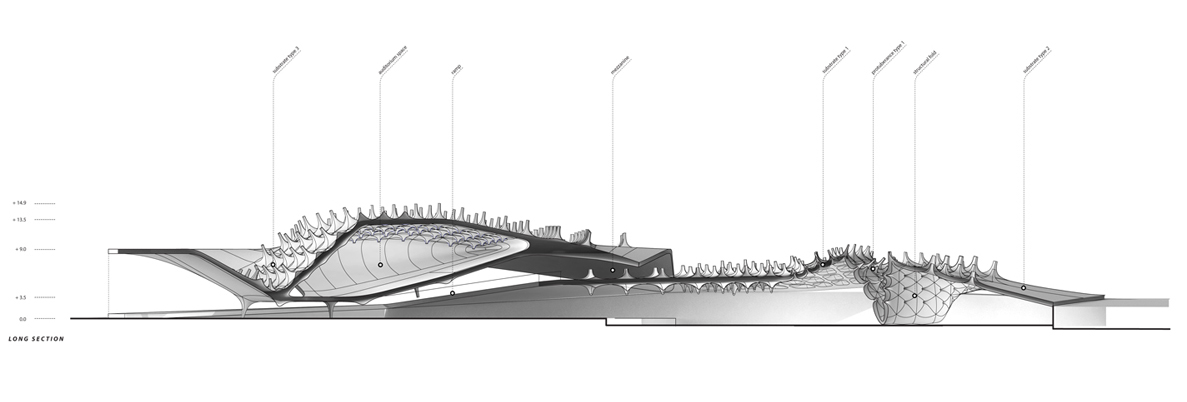
\includegraphics[scale=0.3]{greenroof/7_hydrophile10new}\caption{Global view of the hydrophile}
\end{figure}



\subsection*{Particular aspects}

\newpage{}


\section*{\noun{Christian Derix}, AEDAS Architects R\&D\protect \\
Computationnal Design and Advanced Spatial Modeling}


\subsection*{1 Context of the work of Aedas R\&D}

The company proposes to its client powerful applications of computational
design and advanced spatial modeling to design problems, oriented
towards sustainable solutions.

The models that are created can be at several different space scales,
but also include people and their interactions between them and with
their environment ; that can be seen as the switch from original space
syntax to computational models for social logic {[}\textit{Note :
In fact, Aedas does in that case nothing more than complex social
system modeling and analysis, but according to their client profile
that are architects and designers, they market it as an evolution
of space syntax}{]}.

Examples of outlines of different projects are shown on figure {[}{]}
(from \cite{AedasWeb}).

\begin{figure}[h]
\hfill{}\subfloat[Modeling of solar repartition for towers in Abu-Dhabi]{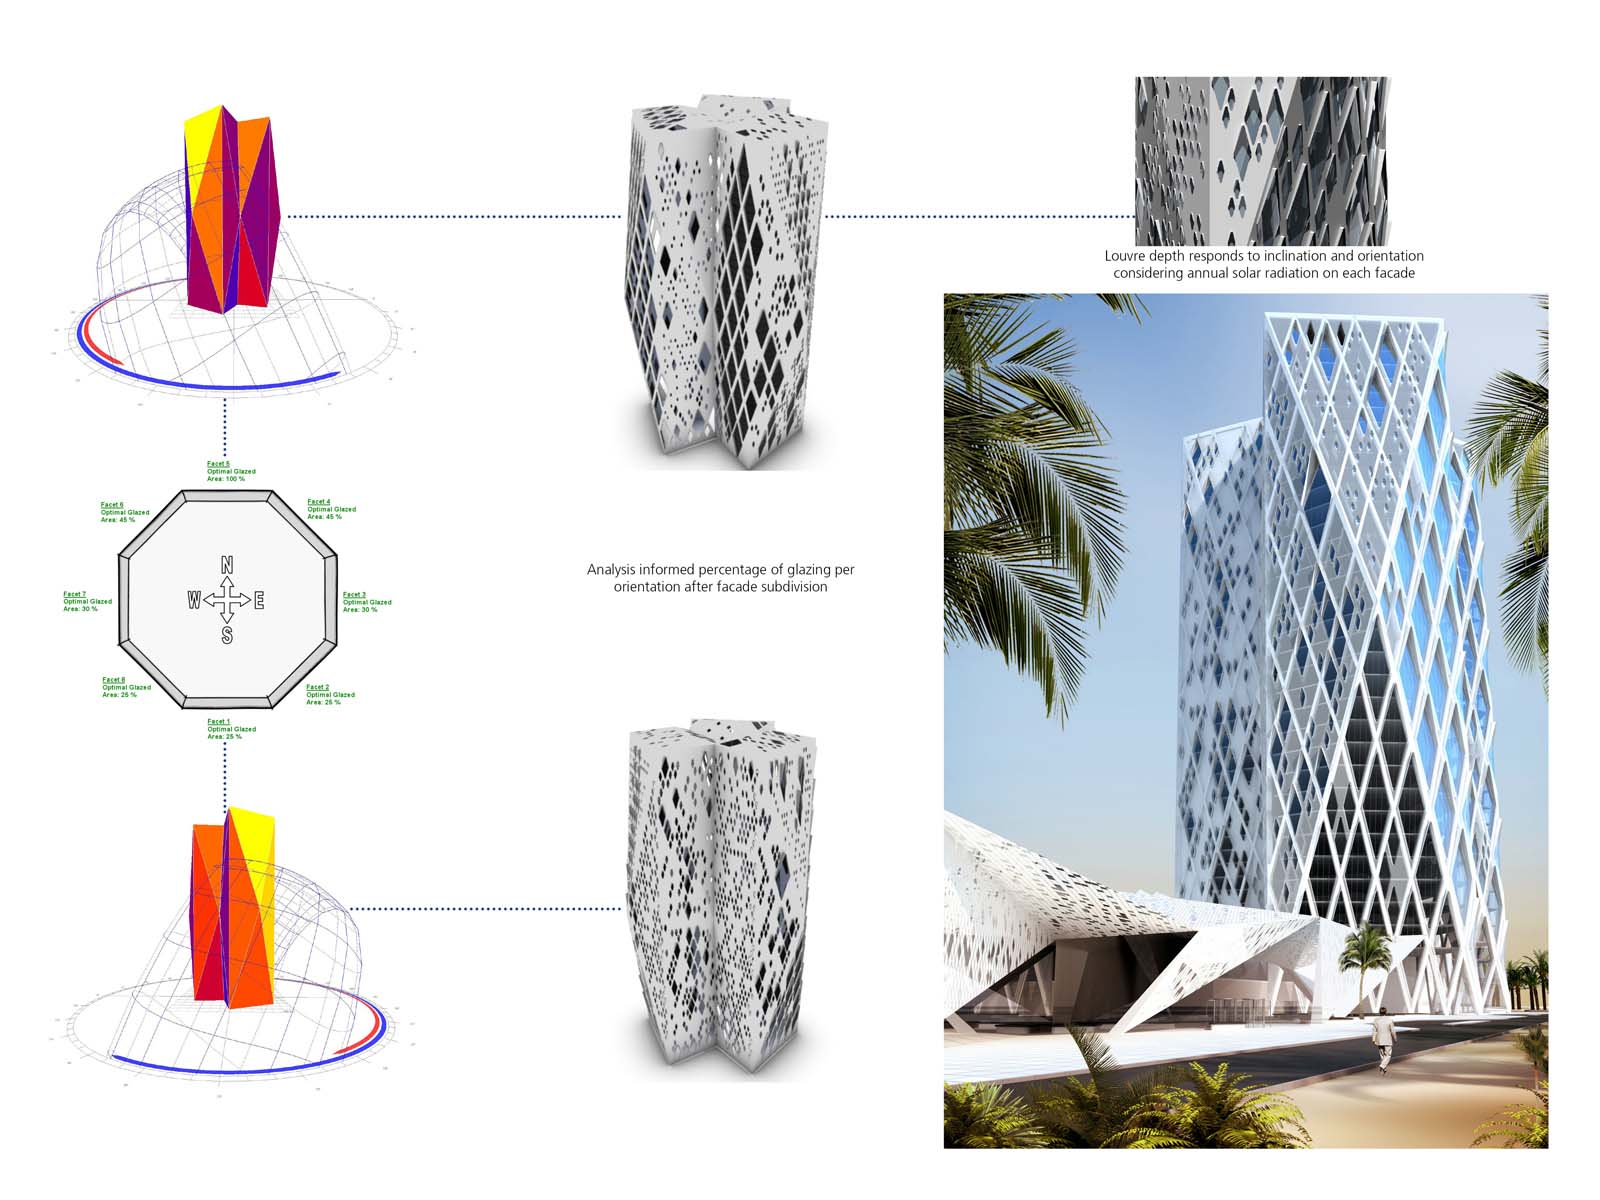
\includegraphics[scale=0.35]{aedas/Cladding-by-orientation-Abu-Dhabi-UAE-ResearchCladding-by-orientation-697}

}\hfill{}\subfloat[Mapping of cycling flows]{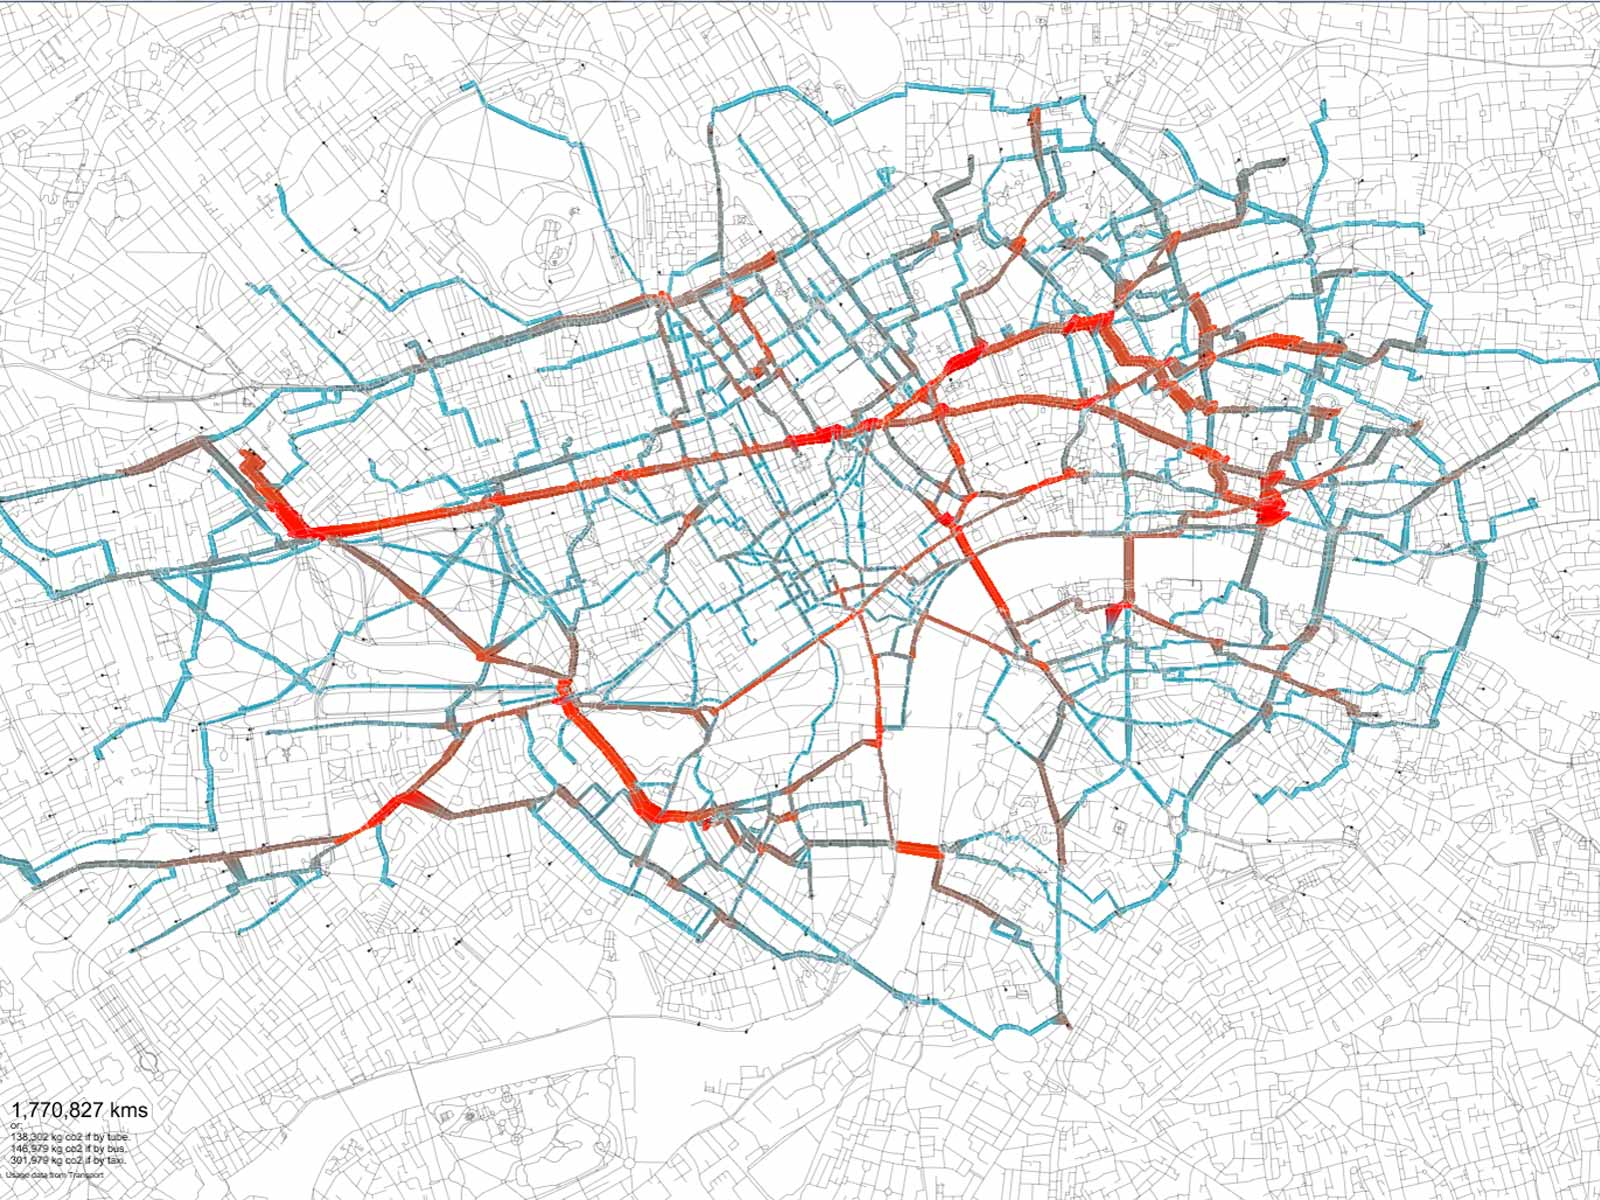
\includegraphics[scale=0.09]{aedas/Cycle-to-Cannes-2011-London-ResearchCycle-to-Cannes-2011-897}}\hfill{}\hfill{}

\hfill{}\subfloat[Global spatial planning solutions]{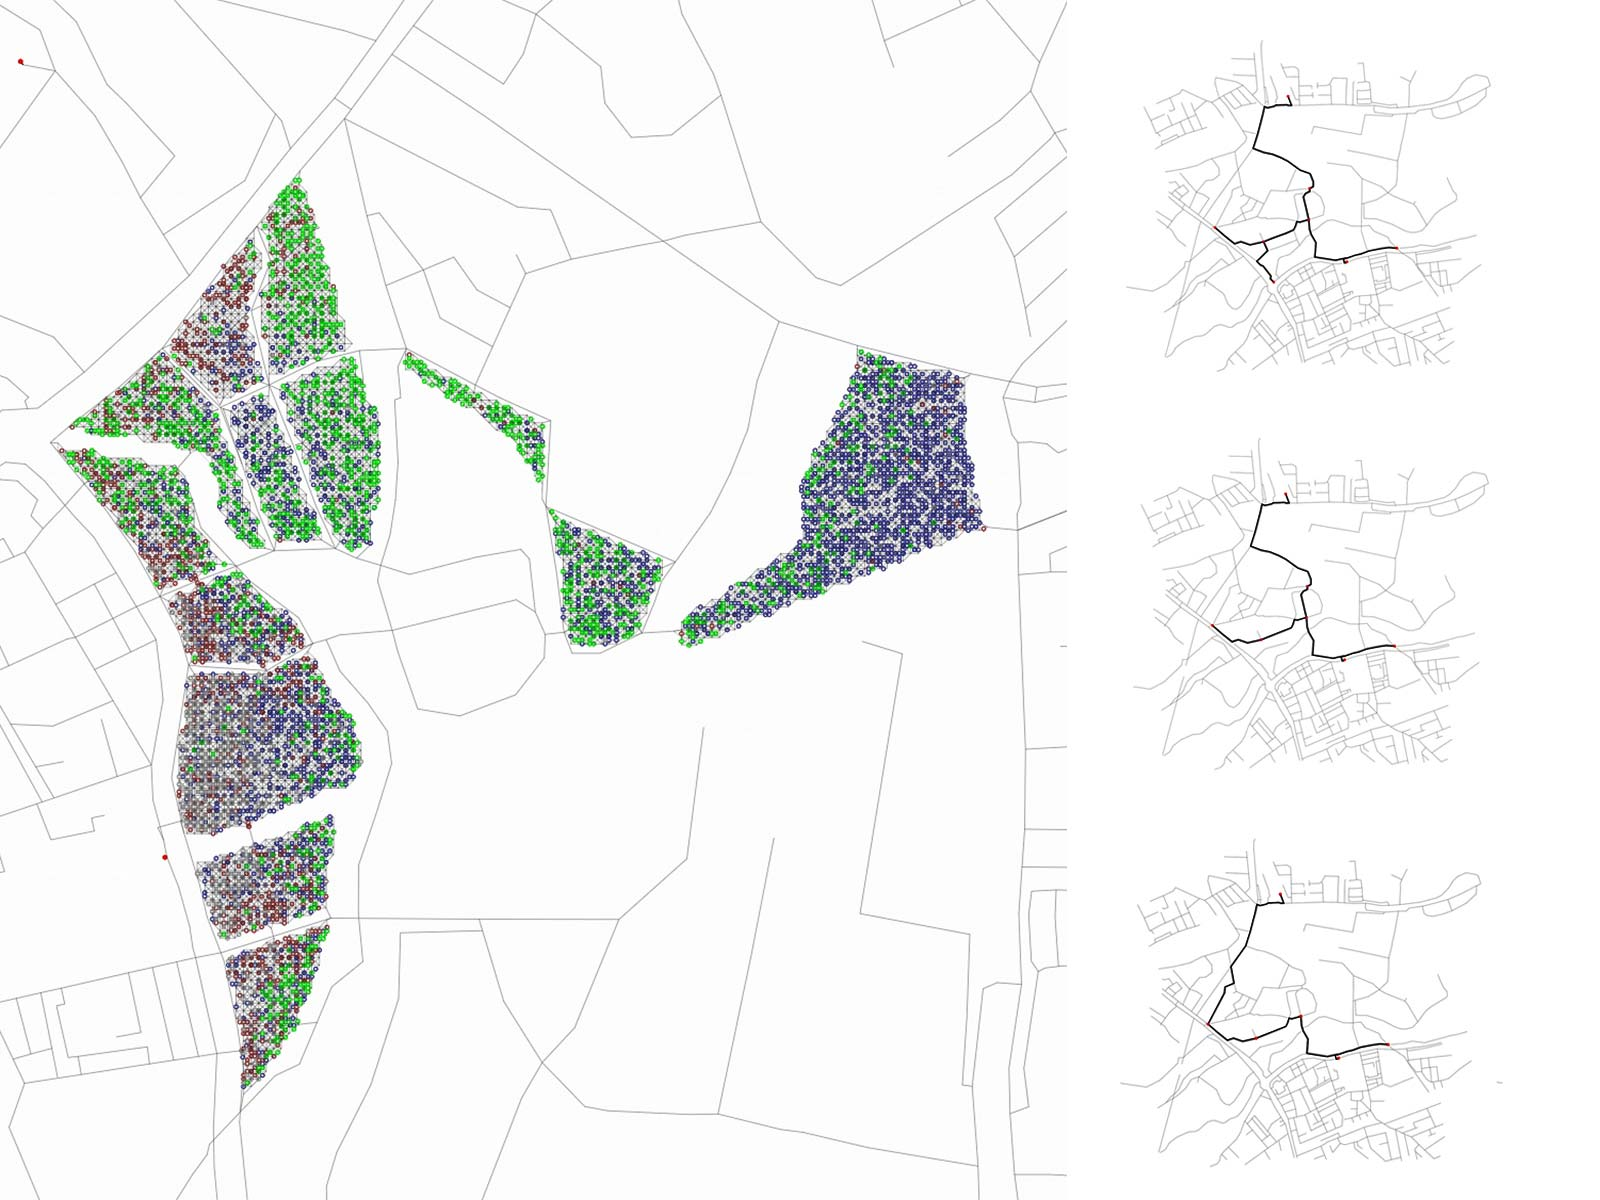
\includegraphics[scale=0.09]{aedas/Smart-Solutions-for-Spatial-Planning-London-UK-Research}}\hfill{}\hfill{}\caption{Results of Aedas projects}


\end{figure}



\subsection*{2 Examples of recent research projects}


\subsubsection*{Study for masterplan}

It is possible to apply directly syntax to help design ; this example
of project shows how a proposal of masterplan is done and how the
designer can move pieces of it to see the consequences through the
self-organisation of the rest of the plan. The modification can be
done at different scales, from furnitures sometimes to the overall
floor.

The techniques used are ``agent-based aggregation'', what seems
to be a computational design of possible configuration (not more precisions
since it appears to be confidential for the company).

The figure {[}{]} shows the final result for the Hong Kong polytechnic
University, after the created masterplan has been integrated to the
other sections.

\begin{figure}
\hfill{}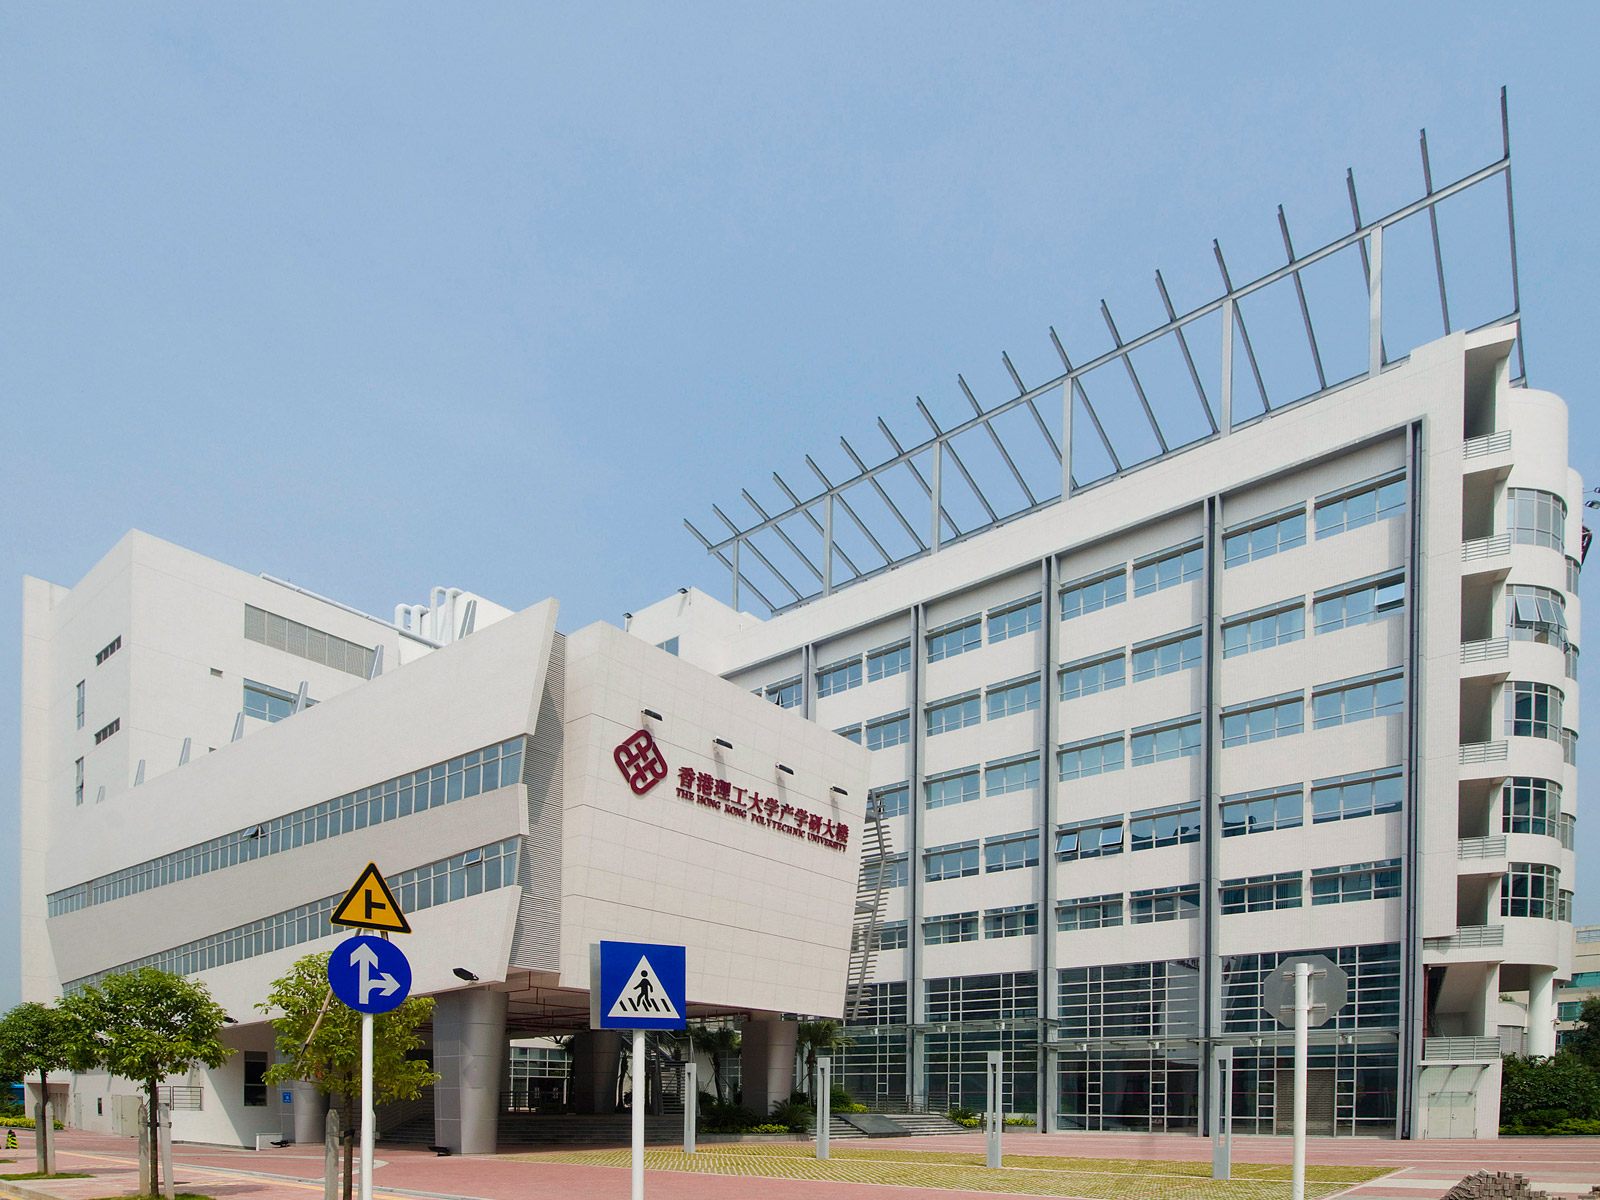
\includegraphics[scale=0.16]{aedas/Hong-Kong-Polytechnic-University-Shenzhen-Campus-PRC-1-671}\hfill{}\hfill{}\caption{Hong-Kong southern Polytechnic University}


\end{figure}



\subsubsection*{Distribution of densities}

For the planning of a new business district in China, there was the
need to decide the local densities of activities (in order to then
directly apply it to the local design of buildings). For that, a tool
was created, that allowed the designer to fix some points at a given
density and observe the generated global field of density that resulted
from these imposed values.

The method used to extract the interpolating field seems to be not
far from non-parametric estimation (see \cite{tsybakov2004introduction})
: with $n$ given points $(M_{1},...,M_{n})$ in space and the expected
values $(y_{1},...,y_{n})$, the problem is to find a function $f$
such that for all $i$, $f(M_{i})=y_{i}$. That can be done for example
by kernel estimation aggregation.


\subsubsection*{Visibility study}

The construction of the new huge tower on the right bank of the Tamise
in London has raised interrogations about its impact on the visual
landscape of the city. The aim of that project was to model the visual
impacts of that new landmark.

To do that, it is possible to calculate by ray-tracing if the tower
is visible from a given point, what was done for a big part of the
city for which the 3D data of building shapes were available. Then
for each point, we can judge if the visible impact is significant,
and also see the total proportion of places for which it has a real
impact.


\subsubsection*{Pedestrian traffic analysis}

For the construction of a new railway station, the locations of entries
for pedestrians had to be decided and a pedestrian flow simulation
model was created.

Concretely, it is an easely parametrizable model, for which test could
be done on localization of ``source'' and ``sink'' points for
pedestrian flows. From an external points of view, it is quite similar
to the problem of distribution of densities, although here the interest
is more on the flow quantities resulting from fixed potential points.
But the method to solve the problem is exactly at the opposite, since
for densities it was solved by a top-down calculation, by global mathematical
calculations, and here the model used is a bottom-up approach, since
it simulates the flows through individuals agents that are the pedestrian
themselves.


\subsubsection*{Mapping architectural controversies}

Urban studies are also sociological studies, as this project testify.
Through newspaper articles analysis, it was possible to proceed to
``social mapping'', and identify trending subjects and social clustering
around these key subjects.

What is really interesting is to make the parallel between the social
system and the architectural system analysis.


\subsection*{Questions}

Question : Do a global comparative knowledge emerge from all these
research projects?

Question : Was network self-generation already considered in one of
the projects?

\newpage{}


\section*{\noun{{\aa}smund Izaki}, AEDAS Architects R\&D\protect \\
Algorithmic aspects of spatial analysis}

That last presentation is a short overview of computer science issues
that occur when doing spatial analysis and investigative modeling.


\subsection*{Complexity of algorithms}

When doing computations, the speed depends on the machine on which
they are done, but what is really important is the intrinsic complexity
of the used algorithm. For example, there exists many ways to sort
a set of number, and the best ones (quick sort or fusion) will have
a mean complexity in $O(n\cdot ln(n))$, what can be assimilated to
a linear time as a function of the size of the set, whereas bad ones
will execute in $O(n^{2})$, what is quadratic and can quickly lead
to impossible calculation times on big data.

This aspect is particularly important in spatial analysis because
of the size of the data and the natural complexity of graph exploration
problems, that's why finding ``good'' algorithms for spatial analysis
is necessary.


\subsection*{Difficulty of problems}


\subsection*{Examples of applications}

\newpage{}


\section*{Conclusion}

The architectural solution for a project is a particular response
to the context of the project, a local proposal in space and time,
but it is also a proposition for architecture in general. Architectural
theory builds itself from concrete responses to concrete cases

\newpage{}

\bibliographystyle{plain}
\bibliography{ArphMorph}

\end{document}
